\documentclass[10pt]{article}
\voffset=-50pt
\hoffset=-90pt
\textwidth= 500pt
\textheight= 625pt
\usepackage[lined,boxed,commentsnumbered]{algorithm2e}
\usepackage{framed}
\usepackage{graphicx}

\newcommand{\myname}{Harjot Gill, Tiernan Garsys, Sam Raper}

\renewcommand{\labelitemi}{$\bullet$}
\renewcommand{\labelitemii}{$\bullet$}
\renewcommand{\labelitemiii}{$\bullet$}
\renewcommand{\labelitemiv}{$\bullet$}

\usepackage{fancyhdr}
\pagestyle{fancy}

\lhead{
  {\bf CIS 700 Airplanes Group 2 Report}\\*
  \myname 
}

\newcommand{\comment}[1]{}

\newcommand{\ms}[1] {
  \texttt{#1}
}

\title{Airplanes Group 2 Report}
\author{\myname}

%%%
\begin{document}
\pagestyle{empty}
\maketitle

%%%
\newpage
\pagestyle{fancy}
\setlength\headheight{60pt}
\setcounter{tocdepth}{3}
\tableofcontents

%%%
\newpage
\section{Introduction}

The goal of this project was to create a strategy to efficiently schedule and control aircraft. While avoiding collisions was obviously the most important goal of the project, delivering all planes to their destination in as few steps as possible proved to be a suitable metric in measuring effectiveness. Our player was given the departure times and destinations of all planes but little other information. Using only these two pieces of information, we strove to quickly deliver all planes. While in the air, planes were not permitted to be within five units of each other.

Throughout the project two important additional challenges were provided. The first was a specific kind of board, which we will refer to as a ``flow board''. On these boards singular planes were not simply flying to various destinations. Instead, there were large numbers of planes departing and going to the same place. It quickly became apparent that a conventional strategy was not sufficient in satisfying these boards.

The second challenge presented was dependencies. In this case, some flights were dependent on the succesful arrival of one or more other planes. This too proved to require additional changes to our initial implementation.

%%%
\newpage
\section{Initial Insights and Observations}
When we first started working on this project, our initial intuition was to
solve the problem at a single-agent level without doing any sort of
pre-calculation or simulation; one would simply need to develop some simple
rules for directing the airplanes toward their goal while avoiding other
airplanes, and the rest should fall into place. Our initial implementation, to
this end, was a simple agent wherein each plane would be influenced by a ``force
vector'' at each timestep, similar to a ``boid'' simulation seen in computer
graphics. The basis for this force vector would be a vector pointing from the
plane's current location to its destination. At every time step, one would
modify this vector by adding a ``repulsive'' vector pointed away from any nearby
planes or walls. Once the final vector was calculated, the plane would maneuver
toward this vector unwaveringly. \\\\

Additionally, we made the insight (along with several other groups) that the total runtime for
any particular map was bounded by the maximum across all planes $P$ of $distance(P_{source}, 
P_{destination}) + P_{departure time}$. In light of this, our initial vector implementation 
contained a prioritization mechanism wherein planes which would land later in an ideal solution
were granted precedence when deciding which plane maneuvered out of the way during collision 
scenarios.\\\\
Upon testing our player, it became apparent that our initial approach was insufficient for this
problem. While scenarios with very few planes were solved easily, the scaling of the problem to
maps with tens of airplanes would result in frequent collisions as planes attempts to avoid one
another would inevitably result in collisions with other planes within the simulation. This 
limitation primarily arose from the fact that each agent only considered the immediate state
of the board at each timestep, disregarding both the implications of its potential move and
the potential actions of all other planes in the simulation; by disregarding such information,
it was easy to fall into cases where the ``optimal'' actions taken by any two individual planes 
in the simulation would lead them to a course which was uncorrectable, and thus would result in
a collision. From this, we realized that a more unified, intelligent strategy was necessary to
succeed.

%%%
\newpage
\section{Strategies \& Concepts}
In a radical shift from our initial strategy, we ultimately decided on a strategy that involved
the pre-calculation of flight paths prior to launch. The various aspects of this strategy are 
outlined below.

\subsection{Launch-Time Simulation and Pathfinding}
Instead of attempting to calculate the flight path of a plane dynamically in the air, our final
solution instead set the flight path of a plane once and let it run its course. Once a plane $P_i$'s 
(the i'th plane to depart in the current session)  departure time has been reached in the session, 
the player will begin simulating this plane's path to the destination as follows...
\begin{itemize}
  \item Simulate a path between $P_i$'s source and destination, considering the presence of 
    $P_0$...$P_{i-1}$'s pre-calculated paths with a set of obstacles. On the first iteration, 
    this will be a straight-line path between $P_i$'s source and destination, as no obstacles
    will have been recorded.
  \item If $P_i$ reaches its destination successfully, then set that as the path for $P_i$ in this
    session and launch it. $P_i$ will follow this path until the end of the session.
  \item If $P_i$ experiences a collision during the simulation, then restart the simulation. On this new
    simulation, add an obstacle for the pathfinding where the collision took place.
\end{itemize}

\subsection{Flow Detection}
In response to the trend of ``flow'' boards that arose during this project, our team added a special
``flow detection'' routine during the training phase of the player. If, during training, the player noted
the existence of a ``flow'' on the board (a sequence of five or more planes which approximately shared 
their source, destination, and departure time), then the simulator would, instead of generating a path
as outline above, generate a serialized path where planes would be dispatched in a single-file line
from the flow source to the flow destination.

It became quickly apparent that in the special case of flows a separate approach need be taken. We define a flow as 5 planes departing from the same airport at the same time and going to the same place. While identifying these flows was fairly simple, defining their behavior proved to be more interesting. As flows were in play on the board for much longer than a single airplane, picking a path that was both quick and unobtrusive was extremely important. The problem here lay in the fact that a single flow could obstruct a large amount of other planes so it could not simply be given a higher priority. However, flows were often the last planes to land so giving them ample time to land was equally important.

Our strategy for dealing with these flows once we identified them was essentially to treat them like walls as their steady stream of airplanes would effectively block all other activity in their area. To do so we simply added to the set of walls used by our A* object. These walls were then used for calculating paths for lone planes as well as additional flows. Unlike the lone plane paths, the flow paths were not time sensitive and would thus be considered at every step of simulation.

We found that one of the most important considerations when scheduling our flows was the number of planes in the flow. As our primary metric for evaluating our strategy was total number of steps, we found that prioritizing the flows with a large number of planes was important. In the cases of ties we simply gave precedence to the flow with shorter distance. This may seem counterintuitive longer flows will obviously take a longer time to land. However, in testing, we found that the shorter flows were much less problematic than the longer ones. As long flows often have to go across a large part of the board, they would effectively put a wall across a very important part of the board that disrupted many of the other planes, including some of the shorter flows. These flows would have to grow their paths unnecessarily large to avoid the larger flow. In practice, this was not worth it.

%%%
\newpage
\section{Implementation}

\subsection{Flight Plan Determination}
At each call of the \ms{updatePlanes()} method, our solution will iterate through the collection of 
planes and perform the appropriate update action based on its current status within the session.
\begin{itemize}
  \item For each plane that has not taken off, we calculate a flight plan using
    the pathfinding implementation described below, which ultimately returns a
    \ms{List<Waypoint>} representing the waypoints that must be traversed by the
    plane on the way to its destination. The plane is then dispatched heading
    toward its first waypoint.
  \item For each plane that has taken off, check its current bearing and
    location relative to its current waypoint. If it is within a certain radius
    of its current sought \ms{Waypoint}, pop that \ms{Waypoint} off the front of
    the list and take the next \ms{Waypoint} in the list to be the current
    \ms{Waypoint}. If the plane's bearing is directed toward its current
    \ms{Waypoint}, then maintain course; else, turn the plane either
    \ms{TURN\_RADIUS} or $Angle(Current Bearing, Goal Bearing)$ degrees
    (whichever is smaller) toward the current waypoint. 
\end{itemize}

\begin{algorithm}
  \SetAlgoLined
  \DontPrintSemicolon
  \SetKwProg{Fn}{Function}{ is}{end}
  \Fn{A*(start,goal)}{
    $closedset\leftarrow EmptySet()$ \tcp*[h]{The set of nodes already
    evaluated.}\;
    $openset\leftarrow \{start\}$ \tcp*[h]{The set of tentative nodes to be
    evaluated, initially containing the start node}\;
    $came\_from\leftarrow EmptyMap()$ \tcp*[h]{The map of navigated nodes.}\; 

    $g\_score[start]\leftarrow 0$ \tcp*[h]{Cost from start along best known
    path.}\;
    \tcp*[h]{Estimated total cost from start to goal through y.}\;
          $f\_score[start]\leftarrow g\_score[start] +
          heuristic\_cost\_estimate(start, goal)$\;
           
          \While{$openset.empty()$ $!=$ $true$}{
            $current\leftarrow openset.leastFScoreNode()$\;
              \If{$current$ $==$ $goal$}{
                \emph{return reconstruct\_path(came\_from, goal)}\;
                }
              
              $openset.delete(current)$\;  
              $closedset.add(current)$\;
              \ForEach{element $neighbor$ in neighbor\_nodes(current)}{
                  $tentative\_g\_score\leftarrow g\_score[current] +
                  dist\_between(current,neighbor)$\;
                  $tentative\_f\_score\leftarrow tentative\_g\_score +
                  heuristic\_cost\_estimate(neighbor, goal)$\;
                  \If{$closedset.contains(neighbor)$ $==$ $true$ $\&\&$ $tentative\_f\_score$
                  $>=$ $f\_score[neighbor]$}{
                    \emph{continue}\;
                        }

                        \If{$openset.contains(neighbor)$ $==$ $false$ $||$
                        $tentative\_f\_score$ $<$ $f\_score[neighbor]$}{ 
                      $came\_from[neighbor]\leftarrow current$\;
                      $g\_score[neighbor]\leftarrow tentative\_g\_score$\;
                      $f\_score[neighbor]\leftarrow tentative\_f\_score$\;
                      \If{$openset.contains(neighbor)$ $!=$ $true$}{
                        $openset.add(neighbor)$\;
                       }
                }
              }
           }
           \emph{return failure}
        }
  \caption{A* Search Algorithm\label{algo:astar}}
\end{algorithm}

\begin{figure}[h!]
  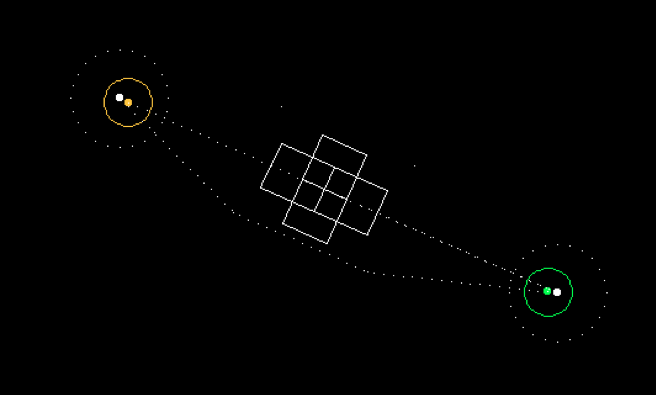
\includegraphics[width=150mm]{wp.png}
  \caption{Ad-hoc virtual obstacles and waypoint Placement}
\label{fig:wp}
\end{figure}

\begin{figure}[h!]
  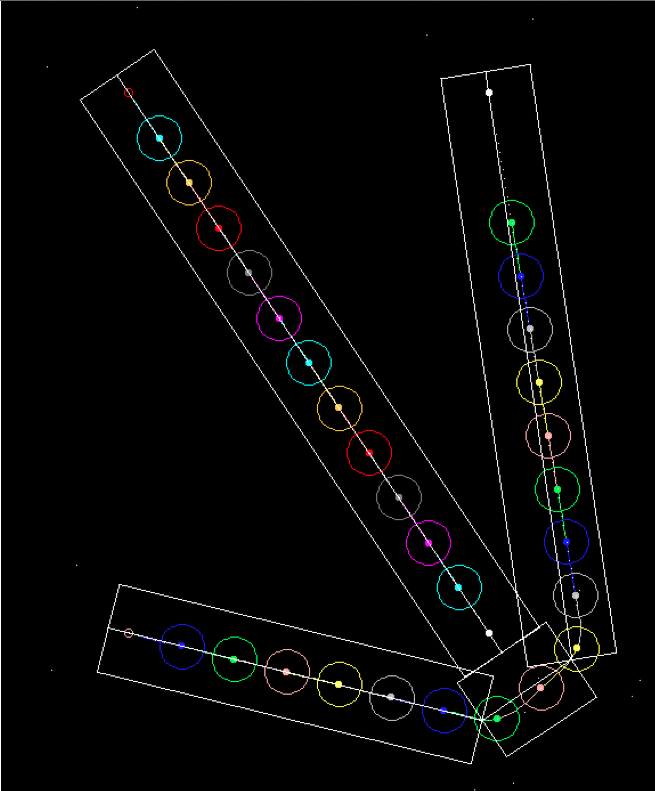
\includegraphics[width=150mm]{diagonal_flows.png}
  \caption{Flow-based virtual obstacles and waypoint Placement}
\label{fig:diagonal_flows}
\end{figure}

\subsection{Pathfinding Implementation}
Pathfinding in our implementation is a time-aware variant of the A* algorithm,
using straight-line distance as a heuristic. Because this heuristic is
admissible (i.e. it never over-estimates the actual distance needed to reach the
goal), one knows that for any particular board configuration it will generate
the optimal path between the source and destination. The procedure for
determining a path is explained in Algorithm~\ref{algo:astar}. Our A-Star
algorithm implementation takes as input a set of waypoint locations on the board
to traverse to get from a source to destination.  The waypoints have to be
placed so that A* is able to find path between any two given points on the board
despite the obstacles and the path distance has to be reasonably close to the
shortest possible distance between these points.  Both these criterion are
satisfied when the waypoints are near the edges of the obstacles. 

In the initial implementation, a collision obstacle resulting from a collision
in a prior simulation would be present in each time step of subsequent
simulations, thus causing all pathing decisions to attempt to move around it. In
subsequent implementation, we implemented that the obstacle would only appear in
timesteps around that in which the collision generating the obstacle occurred,
to simulate the presence of the collided plane at that particular point in
time.\\\\

Figure~\ref{fig:wp} shows a typical obstacle and waypoint placement
configuration from one of the simulation runs. As mentioned earlier, an obstacle
(two perpendicular rectangles resembling a cross) is placed at the collision
point and one of the colliding planes is forced to go around this virtual
obstacle using the four waypoints around this obstacle, so as to avoid "real"
collision. Waypoints were also added in a radial pattern around the airports, so
as to allow planes to take-off in opposite direction than the destination, if
they can. To recap earlier discussion, each (non-flow) plane computes path to
destination before it has taken-off. It simulates (initially) a straight line
flight-path to destination and recursively adds virtual obstacles and reruns the
simulation on detecting collisions with planes which are already in the air.
Care is taken to prevent infinite collision-detection/simulation loop by
enforcing a cap on maximum simulations a plane can run before taking-off, though
this scenario rarely occurs. Also, a limit is placed on the maximum length of
the detour path a plane could choose, so as to prevent unreasonably long paths,
i.e. we observed that sometimes it is better to delay taking-off the planes,
rather than take a long detour.


Figure~\ref{fig:diagonal_flows} shows obstacle and waypoint placement
for group of planes forming "flows". Unlike ad-hoc, real-time approach for
pathfinding before taking-off new planes, the flow planes fly along pre-computed
paths. This closely resembles circuit establishment approach in communication
networks, in which traffic flows along a pre-determined circuit/path. This
approach helps increase traffic throughput especially in scenarios in which

multiple flows intersect each other. As mentioned earlier, the flows are
detected before running the actual simulation and paths/circuits are
pre-computed too. The non-flow planes attempt to fly around the flow-planes
using the normal ad-hoc approach at runtime.



\subsection{Referenced Constants}
\begin{itemize}
  \item \ms{TURN\_RADIUS}: The number of degrees the plane may turn during a timestep. The theoretical limit of 
    10.0 by the simulator was found to cause issues due to floating point imperfections where the simulator would
    crash due to a bearing change of more than 10 degrees, so a value of 9.5 was ultimately used.
\end{itemize}


%%%
\newpage
\section{Results}

Our player did reasonably well in a variety of environments and configurations. As the boards were each quite unique, it may be best to examine them individually. It should be noted that there was an element of nondeterminism in our player when using the A* algorithm. In our implementation, when there was a tie between the length of two paths, the chosen one was selected randomly. While this may seem to be of small consequence, we found that the effects were often quite dramatic. On boards where a lot of these decisions were being made, we could see large swings on various runs. To this end our tournament results should be taken with a grain of salt, although they still contain worthwhile indicators of our performance overall.

\subsection{chaos}

This was by far our worst performance. We can attribute our poor performance on this map to our omission of scheduling flows with dependencies. This map combined three of the most difficult aspects of the project in a way that we did not anticipate. The most step-consuming part of this map was the dependent flows. As we see it, dependencies were more or less a problem of scheduling. To handle heavily dependency-laden maps, we should have implemented a scheduling algorithm that would take into account the depth of a dependency string. To do so, we could’ve created a sort of directed graph in which planes represented nodes and edges represented dependencies. We could then weight the nodes and determine the latest theoretical arrival based on the graph. With this information we would be able to prioritize the most problematic paths and improve our runtime greatly.

With our current implementation, the effect of dependencies was not taken into consideration for the flows at all. On this board two flows were dependent on each other. In Figure R1, you can see the state of the board at step 325. All planes have landed except for a flow going on the same path as the cyan plane and a flow going in the opposite direction. Unfortunately, the flow in the same direction as the cyan plane is dependent on that going the opposite direction so all planes must wait for the cyan plane to land. With the above improvements to our scheduling algorithm, it would have been easily possible to foresee this situation and schedule the cyan plane and all planes on which it depended earlier. 

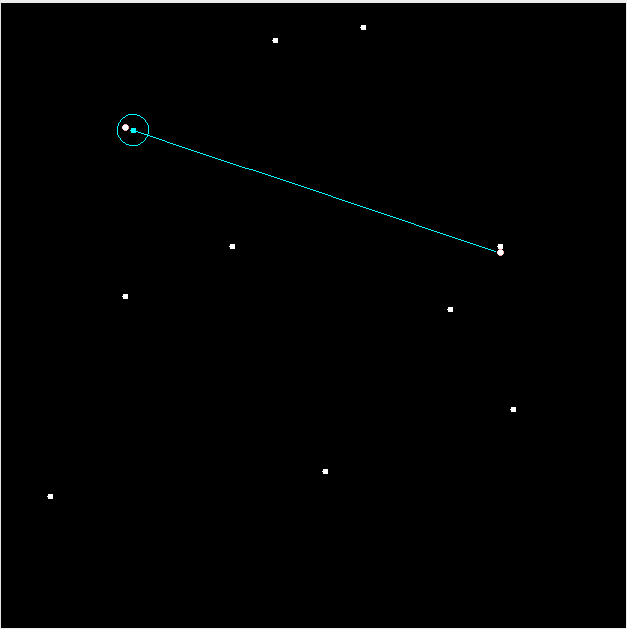
\includegraphics[width=125mm]{pics/R1.png}
\caption{Figure R1: Dodger on chaos.txt board at step 325}

\subsection{DiagonalFlows}

Our performance on Diagonal Flows was quite good. At 711 steps we were less than 50 from the best, 666. The white boxes, shown below in figure R2 demonstrate how the flows were set up. As the flows had the same number of planes and were of exactly equal length, the top-left to bottom-right flow was given priority arbitrarily. It was thus given a straight path and the other flow was forced to work around it. Two waypoints were placed at either end of the straight flow. A* was then used to find a path for the remaining flow using the waypoints set by the straight path. The reason that the flows are wider than absolutely necessary is to account for the turn radius of the planes. If you’ll notice, where the planes are forced to turn around the edge of the flow, the planes deviate from the calculated A* path. In this case, the path could have been tightened up as the bottom flow is giving a slightly wider berth around the bottom-right airport than necessary. This idea of “flow safety” was something that we tried tweaking but ultimately decided to set at a fairly conservative value. While it is appealing to reduce its value on known boards, with the introduction of unknown boards it is paramount to take a safer route.

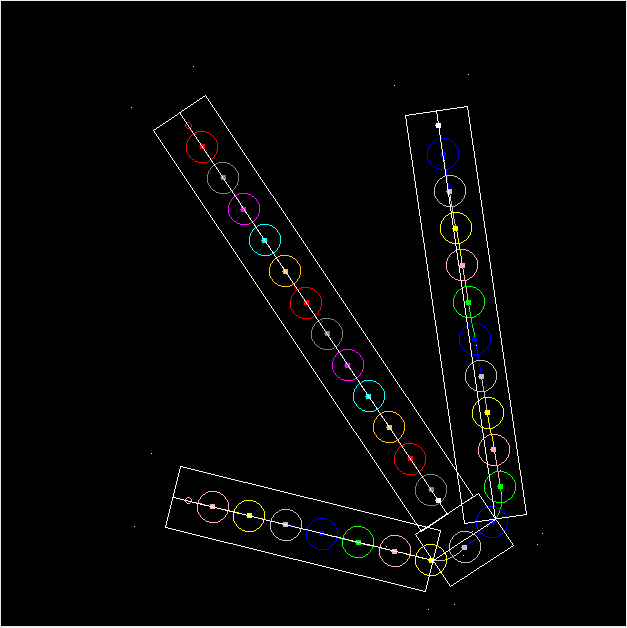
\includegraphics[width=125mm]{pics/R2.png}
\caption{Figure R2: Dodger on DiagonalFlows.txt board}

Another change that could have improved our performance on this and other flow boards is the inclusion of non-uniform paths for flows. In this case such a strategy could have helped in two ways. First, the straight path could have had several arcs rather than a single file line. Doing so would have increased the rate at which the airplanes were departing and arriving, increasing the throughput of the flow. Additionally, the longer path could have been split into a path going as illustrated above and a separate path going around the top of the straight flow. With the airplanes leaving at different angles throughput would again be drastically increased.

Although these improvements could have been made, they would only really be effective on boards similarly simple and unobstructed. Both require the flows to take up more than minimal space, which is a dangerous decision to make. We believe our solution, shown above, was safer in most cases and inoptimal only in the special case shown above.

\subsection{stream}

Our performance on this board was on par with the best score. We completed the board in 165 steps, the best being 153. The part of our strategy that played most into our success on this board was our policy of getting all planes off the ground as soon as possible. In Figure R3 below, you can see that the planes at the top, heading towards the southern-most airports, take off despite the many conflicts that they create, especially with the top and bottom set of flows.

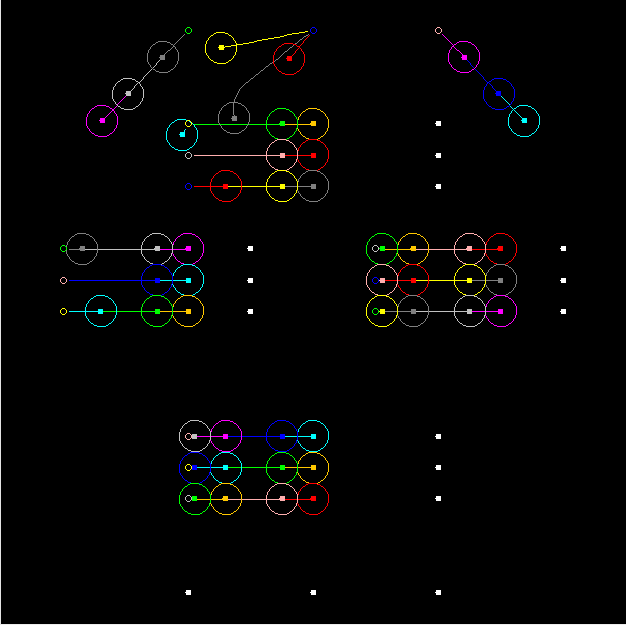
\includegraphics[width=125mm]{pics/R3.png}
\caption{Figure R3: Dodger on stream.txt at step 20}

The flights prove to interrupt the flows but, as they are the most step-intensive flights, it serves to put them in the air as soon as possible. The flows, while they contain a large amount of airplanes, have a relatively short distance to travel and are thus able to recover from the interruptions easily.

The next important thing to notice about our solution to this map is the paths chosen for the flows. Here comes into play our decision to prioritize the shorter distances. The horizontal flows are thus chosen and the vertical flows, which have to traverse the whole board, are forced to adapt. While this creates a relatively long path for the vertical flows, it actually saves time and path length in the long run. Prioritizing the long paths would have created problems for all four of the horizontal flows. The paths for the flows can be seen in Figure R4:

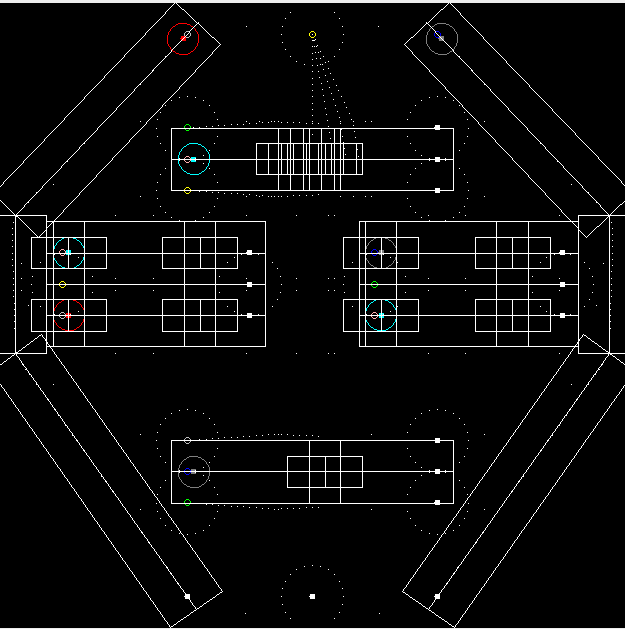
\includegraphics[width=125mm]{pics/R4.png}
\caption{Figure R4: Paths for flows on stream.txt board}

We can see the progression of the simulation in Figure R5 below. While a relatively convoluted picture, there are important takeaways. The right and bottom horizontal flows have finished launching their planes and are no longer a problem. We still have planes to launch in the top and right flows as the planes departing individually from the top have disrupted them. Additionally, we can see our take-off-immediately policy in action by the paths taken from the top middle airport. The planes took off at various angles to increase throughput and the player took care of them as they came. 

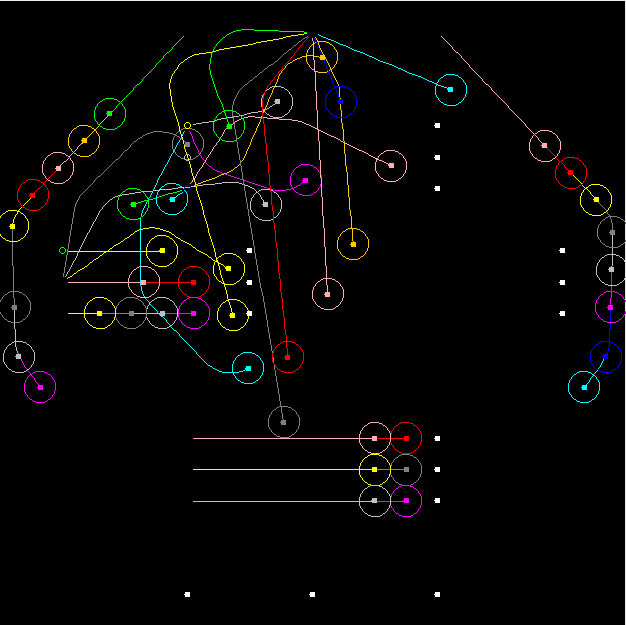
\includegraphics[width=125mm]{pics/R5.png}
\caption{Figure R5: Dodger on stream.txt at step 69}

Finally in Figure R6 below we can see the end of the simulation. As the individual flights reach their destination at the bottom of the board, the rest of the planes in the left and top horizontal flows are able to take off and land. Even though these flows were interrupted by the vertical individual planes, they were not the last to land. We still had to wait for the non-flow planes despite giving them precedence. This board proved how important getting planes in the air early was to our strategy.

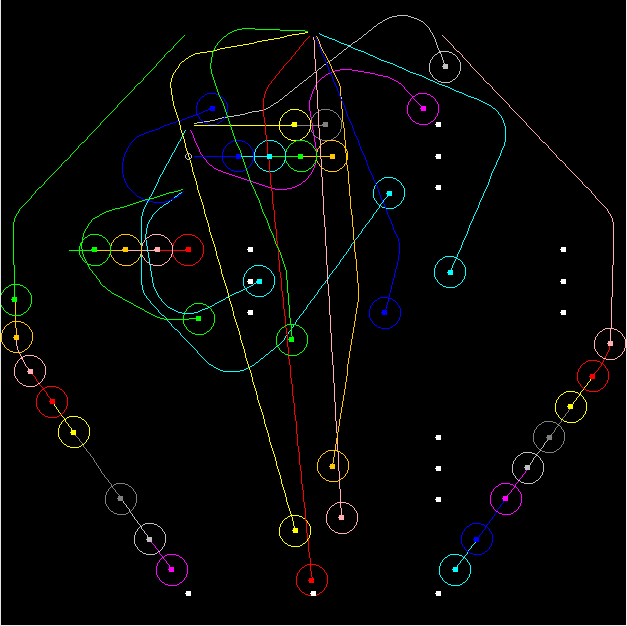
\includegraphics[width=125mm]{pics/R6.png}
\caption{Figure R6: Dodger on stream.txt at step 105}

\subsection{tangle}

Tangle was a dependency board on which our lack of even a simple scheduling algorithm proved to be our downfall. We completed the board in 316 steps while the best in the class was able to do so in 266. Our lack of scheduling and its ramifications can be seen several times throughout the simulation. For the most part, pathfinding on this map was a nonissue as there were not enough flights in the air at any one point to cause many collisions. We can see the first instance of our lack of scheduling in Figure R7.

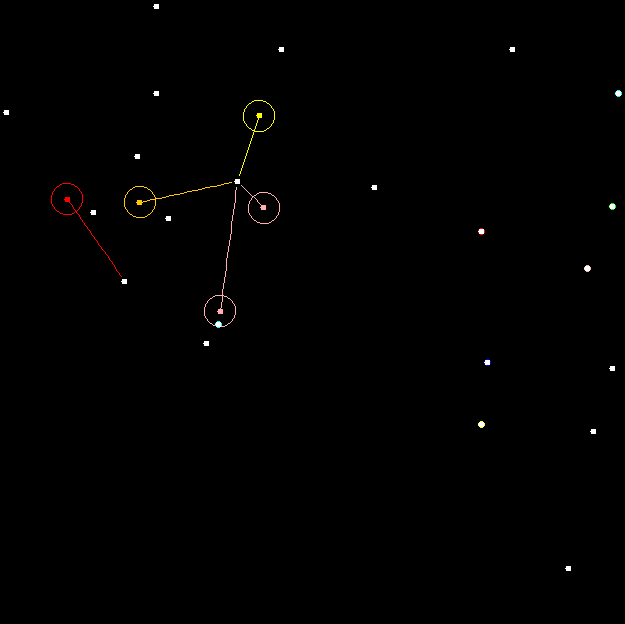
\includegraphics[width=125mm]{pics/R7.png}
\caption{Figure R7: Dodger on tangle.txt at step 118}

All four planes originating from the middle airport were dependent on a single flight and were thus given equal opportunity to leave once it landed. However, the flight heading to the right of the board has much more importance than the others. A long chain of flights, which bounds the optimal time for this board, are all dependent on this flight. For this reason, that plane should have been given precedence and taken off first. However, due to the unsorted nature of our implementation, it was forced to wait for the other three to depart.

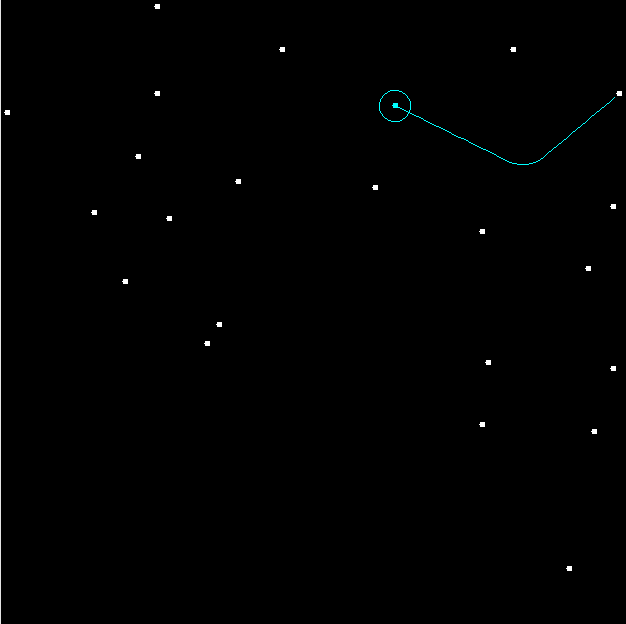
\includegraphics[width=125mm]{pics/R8.png}
\caption{Figure R8: Dodger on tangle.txt at step 296}

This problem persists in Figure R8 above. This cyan plane, although the last plane to land, was forced to dodge a plane that had taken off earlier. Because our planes followed fixed paths once they had taken off, the cyan plane was the only one making decisions. While the sorting solution would have solved this problem, we could also have avoided it by making both planes in a collision eligible for course correction. By running two simulations, one for each plane in the collision and then comparing the land time of both planes in both simulations, we could choose which correction would be most advantageous. This, however, would take an inordinate amount of time on larger boards with more flights. A simple sorting solution would probably be more efficient and easier to implement.

\subsection{Test10airports50flights}

Our performance on this map was not nearly as strong as it could’ve been. Our player was able to land all flights in 159 steps, with 114 being the best in the class. This board presented the challenge of high-density airports. Consider Figure R9 below:

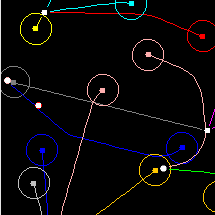
\includegraphics[width=125mm]{pics/R9.png}
\caption{Figure R9: A high-density airport on test50flights10airports.txt board}

The leftmost airport, into which the dark grey plane is flying, is a high-density airport. After the dark grey plane lands, the yellow flies in immediately, and then the light grey from the bottom. This causes the planes on the ground at the airport to delay an unreasonable length of time. As the simulation progresses, we see that the same airport that was so in demand earlier holds the two last planes to land. In this case, our strategy of greedily taking planes off backfires. Each of the planes that needed to land at the high density airport was able to take off quickly at the beginning of the simulation but, in doing so, blocked important planes from departing. An improvement to our player would take into consideration the activity both in and out of an airport when scheduling planes.

\subsection{tight_grid_circle}

Our player performed quite well on this board finishing in 148 steps, only 14 more than the best in the class. An interesting part of our player that this board brings to light is the nondeterministic nature of our solution. Running repeated trials, we were able to finish the board in as few steps as 123 (and as many as 190) as seen in Figure R10:

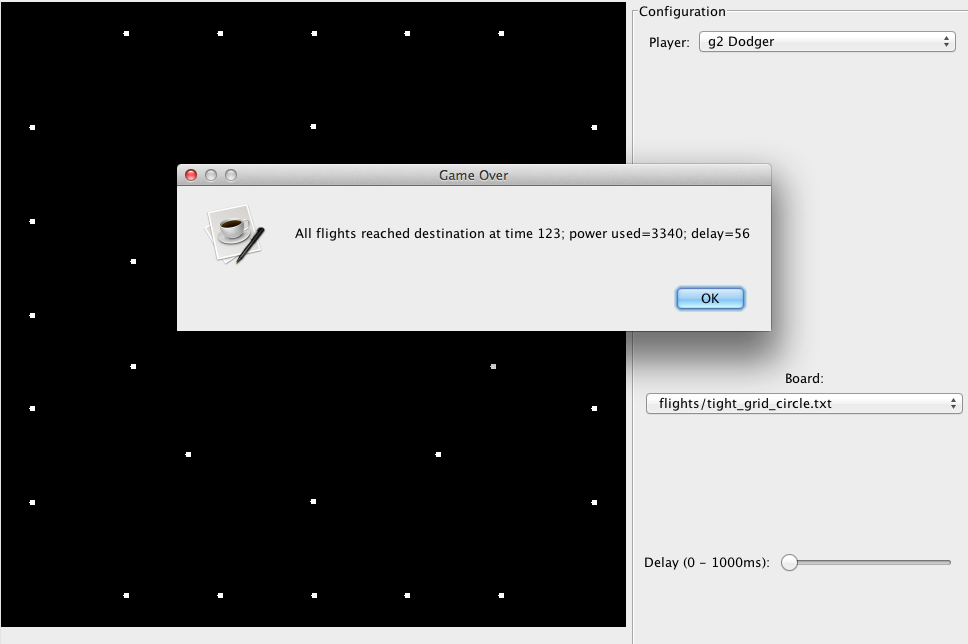
\includegraphics[width=125mm]{pics/R10.png}
\caption{Figure R10: Dodger finishing in 123 steps on tight_grid_circle.txt board}

The reason that we saw such variance on this board in particular was because of the large number of equidistant paths for A* to choose between. The board is basically two sets of planes, the 20 outer, and the 10 inner. Every plane in each group is equidistant from its destination and thus the A* implementation gets to make a lot of random decisions. While it would have been possible for us to choose a metric to choose paths by, it is interesting to see the effect that the randomness has on our runtime. In the best case we beat the current best in the class, in the worst we are nearly the worst.

\subsection{zamBoard}

Our performance on zamBoard was the best in the class. Our player completed the board in 178 steps, 21 steps faster than the next fastest player. This board presented the challenge of unused space. With all of the planes and airports at the center of the board, there was a lot of room to work with if you were simply to take longer paths away from the confluence in the middle. On this board we can again attribute our success to taking flights off as soon as possible and letting A* deal with their paths, even if they are not as direct as they could be. This is illustrated in Figure R11 below, where our use of space is evident:

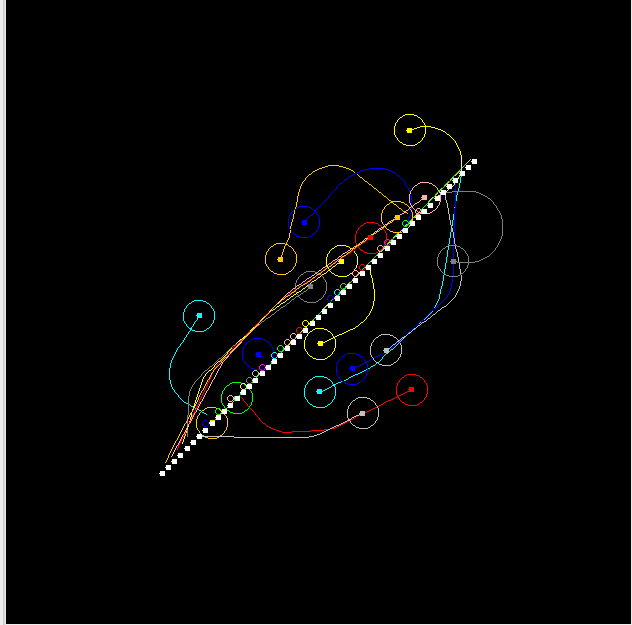
\includegraphics[width=125mm]{pics/R11.png}
\caption{Figure R11: Dodger on zamBoard.txt at step 60}

While not perfect, we are happy how we performed on this board as it was not a case we had thought to optimize for when building the player.

%%%
\newpage
\section{Contributions}

\subsection{Elegant time-aware approach path-finding}

Our approach utilizes time-aware variant of A* algorithm for all scenarios.
There are no hard-coded traffic patterns or behaviors, which makes our approach
very elegant. E.g. plane's take-off and approach angles, in-flight traffic
patterns and even the flows are computed using the A* algorithm. Our
implementation adapted to different board scenarios automatically, and we rarely
had to tweak anything.

\subsection{Tracer implementation}

As part of our testing, we enhanced the simulator to visualize the collisions
and to trace the plane's path finding attempts. This enhancement allowed us to
quickly identify the bottlenecks and helped us to efficiently place the
waypoints.

%%%
\newpage
\section{Future Directions \& Limitations}

\subsection{Flow Optimization}

One minor shortcoming of our solution as presented was its performance 
on so-called ``flow'' boards, characterized by large numbers  of planes that shared 
their source, destination, and departure times and so-named from the serialized 
flow of planes that would form between the source and destination.  While we
were able to improve our performance on these boards by adding flow detection
to the pre-simulation training in the code (implemented by detecting the presence
of five or more planes sharing a source an destination), our solution was limited
by the fact that only one flow of planes was allow between any source-destination
pair. On boards such as \ms{DiagonalFlows} with large amounts of free airspace, Group 5's
player was able to detect the possibility of multiple flows between the source and destination
and subsequently schedule planes to proceed to the destination in two slightly-staggered
flows. While the staggering (necessary for any particular plane to avoid collision with
a plane in another flow immediately at takeoff, before that other plane had cleared the 
airspace) severely reduced the runtime improvements of this strategy, it was nonetheless
better than a one-flow solution; Group 5's player demonstrated a runtime of 666 steps
on \ms{DiagonalFlows}, while our player demonstrated a runtime of 711 steps.\\\\
One could improve on this limitation by adding detection for multiple flow paths between
a source-destination pair during the training phase of our player. Our current implementation
of flow-detection works by finding a shortest path between the source-destination pair, treating
other flows as obstacles obstructing this path. One possibility would be to generate some number
of paths between the source-destination pair, determine which paths are close enough to the
optimal path as to not increase the overall runtime of the simulation after necessary 
staggering was taken into account, and dispatch planes to each of these flows in turn.
Potential implementation difficulties would be being able to determine prior to simulation
that such a splitting would not simply increase the runtime of the entire simulation.

\subsection{Pathfinding Prioritization / Sorting}

Another problem with our solution was the possibility of giving planes whose paths were 
determined last in the sequence of planes overly long paths. As outlined above, our
method of determining paths was greedy in that we would determine the path for any 
particular plane $P_i$ by simply simulating the shortest A* path between the source
and destination of $P_i$ in an environment with planes $P_0$...$P_{i-1}$, resetting
the simulation and trying again with a obstacle placed at the collision point in the
event of a collision. This methodology resulted in a greater number of collisions for the
last planes to have their path decided, which would lead them to be given longer paths to
avoid collisions. Problems arose in that the ordering for resolving plane paths was more-or-less
arbitrary; it was very possible that a plane with a short path in an optimal solution would be
given a longer path, potentially to the detriment of simulation runtime, due to the fact
that it had to consider more obstacles than other planes in determining its final path.\\\\
We attempted to address this problem by prioritizing the order with which planes' paths 
were determined in our pre-flight simulations. Methods tried include...
\begin{itemize}
  \item \ms{Shortest Path First:} Order the planes in ascending order by path length, and 
    resolve flight paths in that order. The intuition behind this was that shorter paths
    would have fewer intersections with other paths, and thus their resolution would generate
    fewer obstacles for later-resolved flights.
  \item \ms{Longest Path First:} Order the planes in descending order by path length, and
    resolve flight paths in that order. The intuition behind this was that longer flights
    are more likely to be the limiting factor in the overall runtime of the simulation, 
    so resolving them first would ensure their runtime would not be increased by collisions
    with shorter flights.
  \item \ms{Least Intersections First:} Determine the straight line paths between all
    source-destination pairs in the simulation. Order the planes in descending order by
    number of intersections with other straight line paths, and resolve flight paths in 
    that order. This method attempted to resolve flights that would be interfered with 
    by many other flights first, thus prevent their runtimes from skyrocketing.
\end{itemize}
In experiments, we found that each of the above methods yielded superior results in different
simulations, with no clear trend of certain strategies working better on certain maps. Due to the
fact that our implementation of sorting was incompatible with our flow detection, our final solution
ultimately scrapped prioritization of plane flights. One issue that would have to be solved if this
were implemented in the future would be gathering useful information for prioritizing flights from
the information that is available at the beginning of the simulation. One only knows when the simulation
starts what the source, destination, and departure time of each plane is. As of time of writing, we 
were unable to find any way of extrapolating from this data a prioritization that would reliably yield
better results on most boards.

%%%
\newpage
\section{Acknowledgments}

\ms{Chris Murphy}, for the awesome class.\\\\
\ms{Tanveer Gill}, for having helped developed the A* package used by our group with Harjot during
the Mosquitos project.

%%%
\newpage
\section{Conclusion}

Overall, this was an extremely interesting and fun project. The opinions of each of the groupmates on
various aspects of the project are below...

\begin{itemize}
\item \ms{T,S,H:}One potential improvement in the future would be to introduce a better metric (or metrics) for success
in this project. As indicated in class, our group felt that the metric of total runtime for the simulation
was flawed, as it made the task too dependent on the performance of the last-arriving plane in the simulation;
as long as they didn't directly interfere with the last arriving plane or delay themselves so much
as to become the last arriving plane themselves, it became less important to optimize the behavior
of other planes. Our group feels a better success metric would be to minimize the sum of total delay and 
total power used over the course of a simulation. By measuring success in this way, the performance of a player
would not be strictly tied to the performance of any single plane, but rather be an aggregate of the performance
of all planes in the session. 

\item \ms{T,S:} Another suggestion for future semesters would be to place the assignment of this project earlier in the 
semester. Having discussed it, we feel that the Airplane problem was a less complicated piece to tackle than Mosquitos, 
due to the simpler goal conditions and fewer factors (no walls, no random agents, etc.) to consider in solving the problem.
By positioning Airplanes earlier, we feel the difficulty of the class would better scale with the time spent in the class. 
In addition, this arrangement would allow more room for extension of the Mosquitos assignment, which could be valuable as 
evidenced by the fact that the Mosquitos problem remained unsolved in an ``ideal'' fashion when we finished with it.


\end{itemize}
  
\end{document}
